% !TEX TS-program = pdflatex
% !TEX encoding = UTF-8 Unicode

%%% DOCUMENT DEFINITION
\documentclass[11pt, french]{article} % use larger type; default would be 10pt
\usepackage[utf8]{inputenc} % set input encoding (not needed with XeLaTeX)

%%% PAGE DIMENSIONS
\usepackage{geometry} % to change the page dimensions
\geometry{a4paper} % or letterpaper (US) or a5paper or....
\geometry{margin=1in} % for example, change the margins to 2 inches all round

%%% PACKAGES
\usepackage{graphicx} % support the \includegraphics command and options
\usepackage{booktabs} % for much better looking tables
\usepackage{array} % for better arrays (eg matrices) in maths
\usepackage{paralist} % very flexible & customisable lists (eg. enumerate/itemize, etc.)
\usepackage{verbatim} % adds environment for commenting out blocks of text & for better verbatim
\usepackage{subfig} % make it possible to include more than one captioned figure/table in a single float
\usepackage[frenchb]{babel}

% Package pour le dessin schéma bloc
\graphicspath{{../Automatique/}}
\usepackage{schemabloc}
\usepackage{amsmath}

%%% HEADERS & FOOTERS
%\usepackage{fancyhdr} % This should be set AFTER setting up the page geometry
%\pagestyle{fancy} % options: empty , plain , fancy

% Rapport projet pluridisciplinaire
% : Xavier Galzin, Stanislas Bertrand, Romain Desille, Frédéric Meslin

\title{Projet pluridisciplinaire : sustentation magnétique}
\author{ Xavier GALZIN, Stan BERTRAND, Romain DESILLE, Fred MESLIN}
\date{30/01/2012}


\begin{document}
\maketitle

\begin{center}
	\vspace{0.6in}
	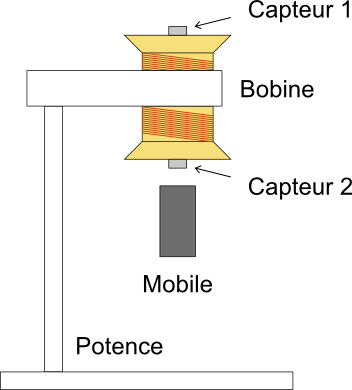
\includegraphics[width=10cm]{Automatique/system_physique.png} 
	\\
	\emph{Le système physique étudié}
\end{center}

\pagebreak

\section{Introduction}
\paragraph{}
	Dans le cadre du projet pluridisciplinaire de cette année, il nous est demandé de faire léviter un mobile dans l'air à l'aide d'un champ magnétique produit par une bobine. On appelle cet effet la sustentation magnétique. Ce projet est une version édulcorée d'un prototype de lampe décorative imaginée par une étudiante de l'école LISAA (Institut supérieur des arts appliqués) et réalisée en partenariat avec des chercheurs et ingénieurs de l'INSA de Rennes.

L'étude demandée présente de nombreuses facettes : il faudra étudier et modéliser le système physique pour ensuite l'asservir à l'aide d'un dispositif d'automatique électronique. Ce dispositif sera réalisé de manière analogique puis de manière numérique. Dans ce rapport, on s'intéressera uniquement à la description du système, sa modélisation et ses constantes prépondérantes ainsi qu'aux correcteurs que nous avons choisi d'implémenter pour maintenir le mobile en lévitation.

\section{Description du système physique}
\paragraph{}

Le système physique est existant et imposé. Il consiste en une potence munie d'une bobine qui servira à exercer le champs magnétique retenant le mobile. La bobine est également munie de capteurs à effet Hall qui permettent, par une mesure différentielle, de mesurer la distance du mobile par rapport à la bobine. On a ainsi la boucle de retour de notre système. 

On a donc finalement une consigne en position que l'on va convertir en un courant qui servira à générer le champs magnétique qui attirera ou repoussera le mobile et le retour en position par le biais des capteurs à effet Hall. 

Le problème principal du système est qu'il n'est pas stable en boucle ouverte. On va donc procéder à une étude basée sur des mesures fournies afin de mettre un place un correcteur qui rendra la système stable. Pour cela, nous poserons les équations mathématiques du problème pour ensuite décrire le modèle de correcteur retenu ainsi que les valeurs des diverses constantes associées à ce modèle.

\section{Modélisation mathématique}

\paragraph{Mise en équation du système}

Forces appliquées sur le système :
\newline

$ F_{bobine} = K \times \dfrac{i^2}{x^2}  $

$ F_{poids} = -m \times g $

On applique le principe de la dynamique :
\newline

$ \sum F_{exterieures}  = m \times {\dfrac{{d^2}x}{dt^2}} $

Linéarisation de la force exercée par la bobine :
\newline

$ {\dfrac{dF(t)}{dt}}_{x = X_0, i = I_0} = \dfrac{\partial F(t)}{\partial x} \times dx + \dfrac{\partial F(t)}{\partial i} \times di $

$ \dfrac{\partial F(t)}{\partial x} = K_x = \dfrac{-2K \times I_0^2}{X_0^3} $

$ \dfrac{\partial F(t)}{\partial i} = K_i = \dfrac{2K \times I_0}{X_0^2} $

Equation différentielle résultante :
\newline

$ m \times {\dfrac{{d^2}x}{dt^2}} = F_{bobine} - m \times g = K \times {\dfrac{I_0^2}{X_0^2}} + K_x \times Dx + K_i \times Di - m \times g $

$ avec : Dx = x - X_0, Di = i - I_0 $

On effectue une transformée de Laplace du système :
\newline

$ m \times x{s^2} = F_0 + K_x \times (x - X_0) + K_i \times (i - I_0) - m \times g $

$ x \times (m{s^2} - K_x) = K_i \times i +(F_0 - K_x \times X_0 - K_i \times I_0 - m \times g) $

$ H(s) = \dfrac{x(s)}{i(s)} = \dfrac{K_i}{m{s^2}- K_x}  $

Etude du point d'équilibre :
\newline

$ \sum F_{exterieures}  = K \times {\dfrac{I_0^2}{X_0^2}} - m \times g = 0 $

$ K = mg \times {\dfrac{X_0^2}{I_0^2}} $

\paragraph{Constantes obtenues par le calcul}

$ K_{bobine} = 1,459 \times 10^{-4} $
$ K_x = 141,7 $
$ K_i = 1,660 $

\section{Correcteur analogique}
\begin{tikzpicture}
\sbEntree{Vxc}
\sbComp{Comp}{Vxc}
	\sbRelier[$Vx_C$]{Vxc}{Comp}
\sbBloc{C}{$K_{p}$}{Comp}
	\sbRelier[$\epsilon_x$]{Comp}{C}
\sbBlocL{E}{$\dfrac{K_{Elec}}{\tau_{Elec} \cdot p + 1}$}{C} 
\sbBlocL{M}{$\dfrac{-\frac{K_i}{K_x}}{-{\tau_{Meca}}^2 \cdot p^2 - 1}$}{E}
\sbBlocL{H}{$K_{Hall}$}{M} 

\sbSortie{Vxr}{H} 
	\sbRelier{H}{Vxr}
	\sbNomLien[0.8]{Vxr}{$Vx_R$} 
\sbDecaleNoeudy{M}{A}
\sbBlocr[0]{A}{$\dfrac{1+ \tau_d \cdot p}{1 + a_d \cdot \tau_d \cdot p}$}{A}
\sbRelieryx{H-Vxr}{A}
\sbRelierxy{A}{Comp}
\end{tikzpicture}

$\tau_d = $


\hspace{1mm} \\ 
\hspace{1mm}\textcolor{green}{\% Paramètres du Système }\\ 
\hspace{1mm} \\ 
\hspace{1mm}\textcolor{green}{\% Modèle Electrique de la Bobine }\\ 
\hspace{1mm}R=2.24; \textcolor{green}{\%Ohm }\\ 
\hspace{1mm}L=1.49e-2; \textcolor{green}{\%H }\\ 
\hspace{1mm} \\ 
\hspace{1mm}\textcolor{green}{\% Modèle d'interaction mécanique de la bobine }\\ 
\hspace{1mm}m=0.1414; \textcolor{green}{\%Kg }\\ 
\hspace{1mm}ki=1.375; \textcolor{green}{\%N.A-1 }\\ 
\hspace{1mm}kx=117.3; \textcolor{green}{\%N.m-1 }\\ 
\hspace{1mm} \\ 
\hspace{1mm}\textcolor{green}{\% Modèle capteur effet Hall }\\ 
\hspace{1mm}Kc\_Hall=92;  \\ 
\hspace{1mm} \\ 



%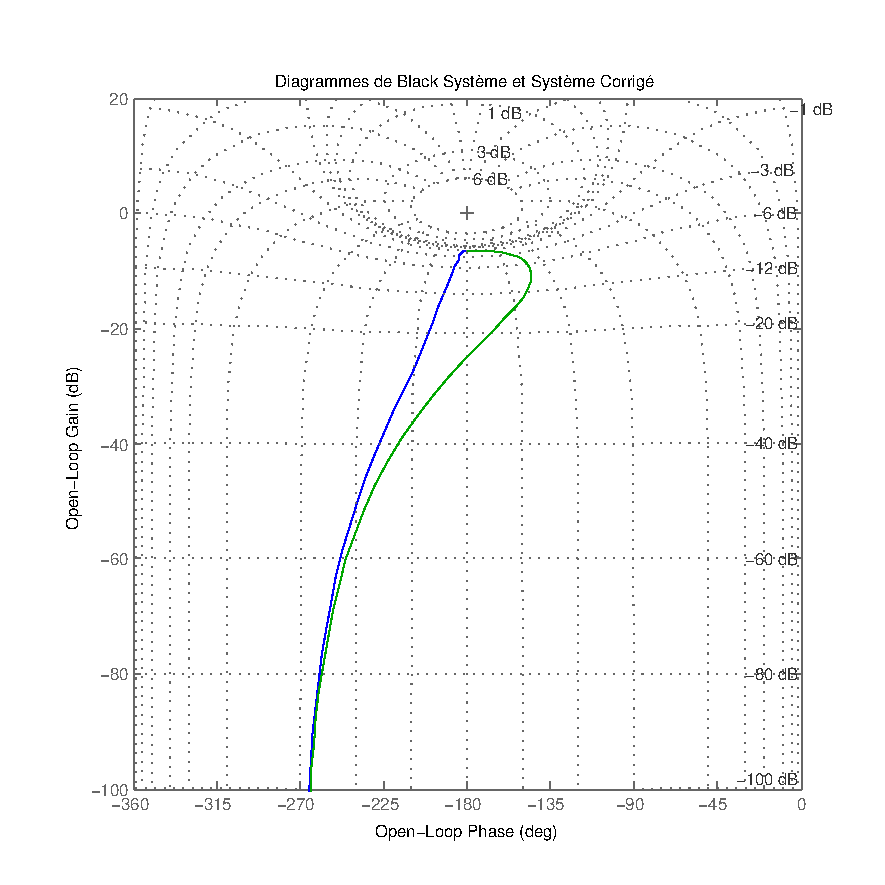
\includegraphics[scale=0.50]{MatBlackFredValues.pdf}
%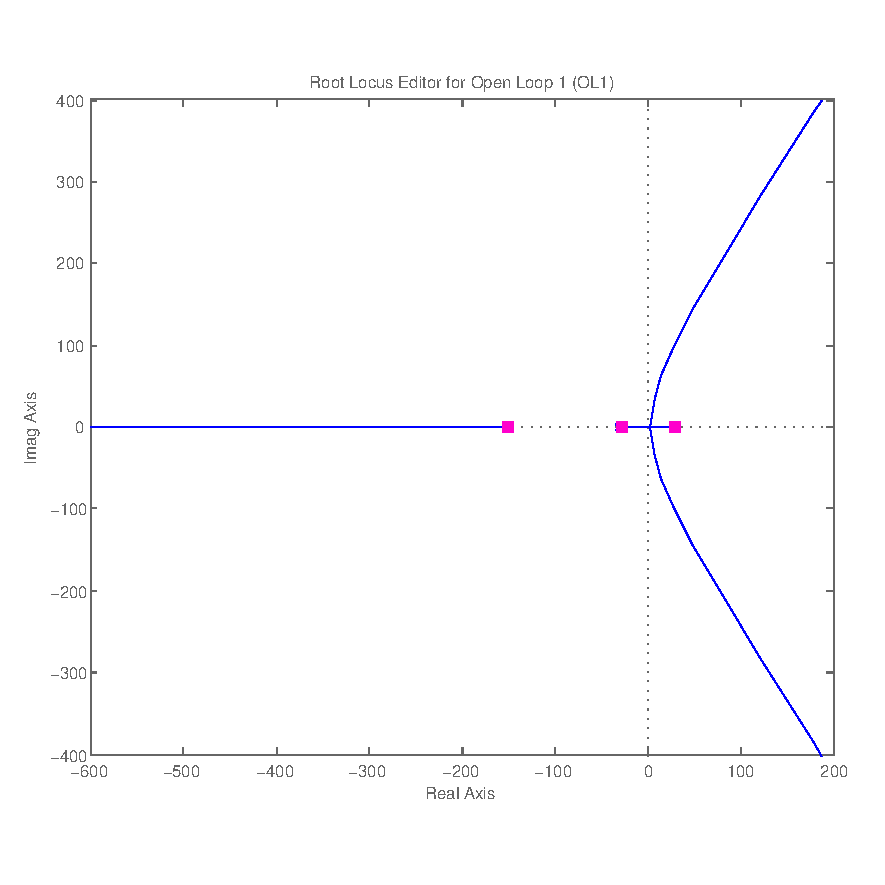
\includegraphics[scale=0.50]{RL_Sys_Seul.pdf}
%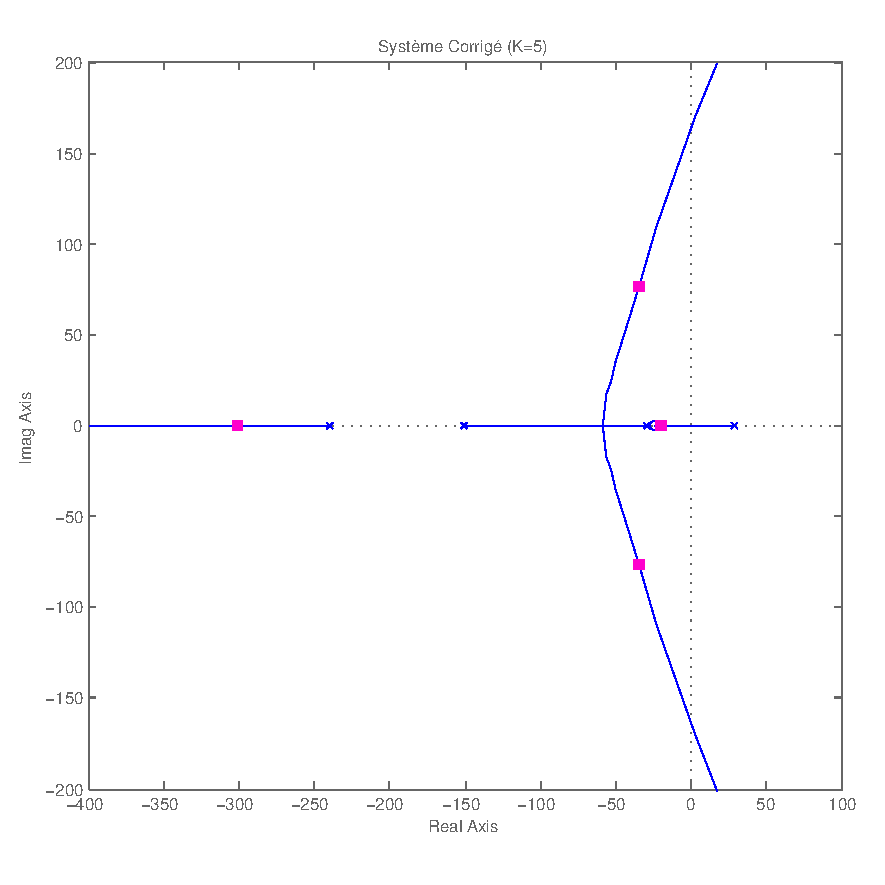
\includegraphics[scale=0.50]{RL_Sys_AvPh_K5.pdf}
%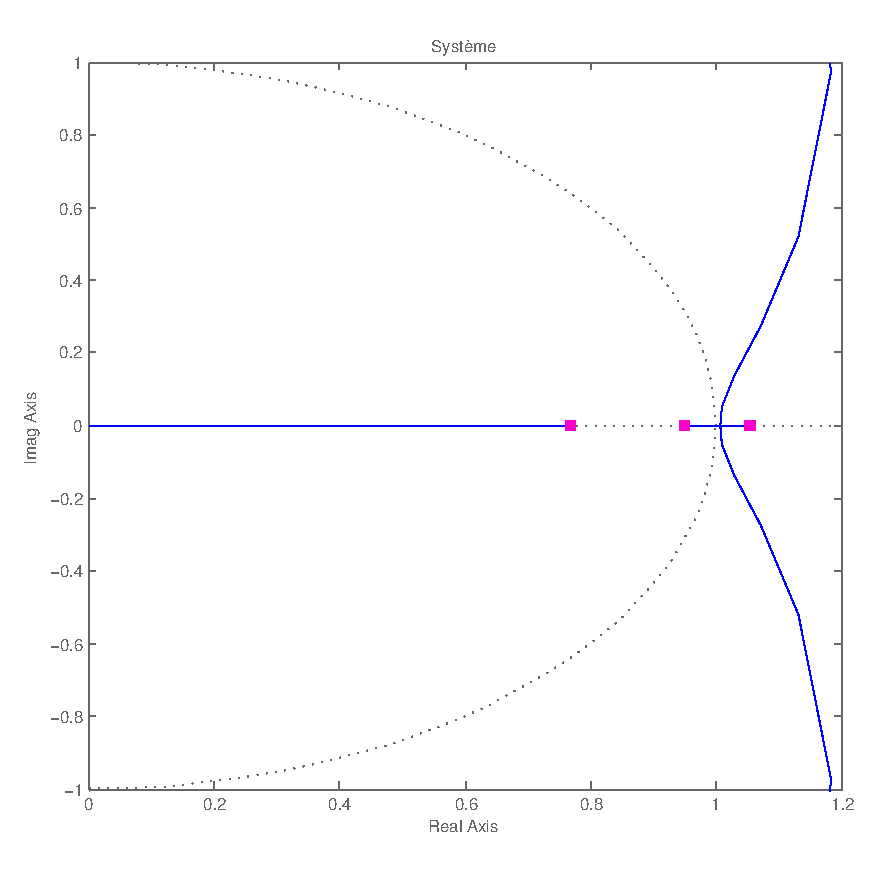
\includegraphics[scale=0.50]{RLN_Sys_Seul.pdf}
%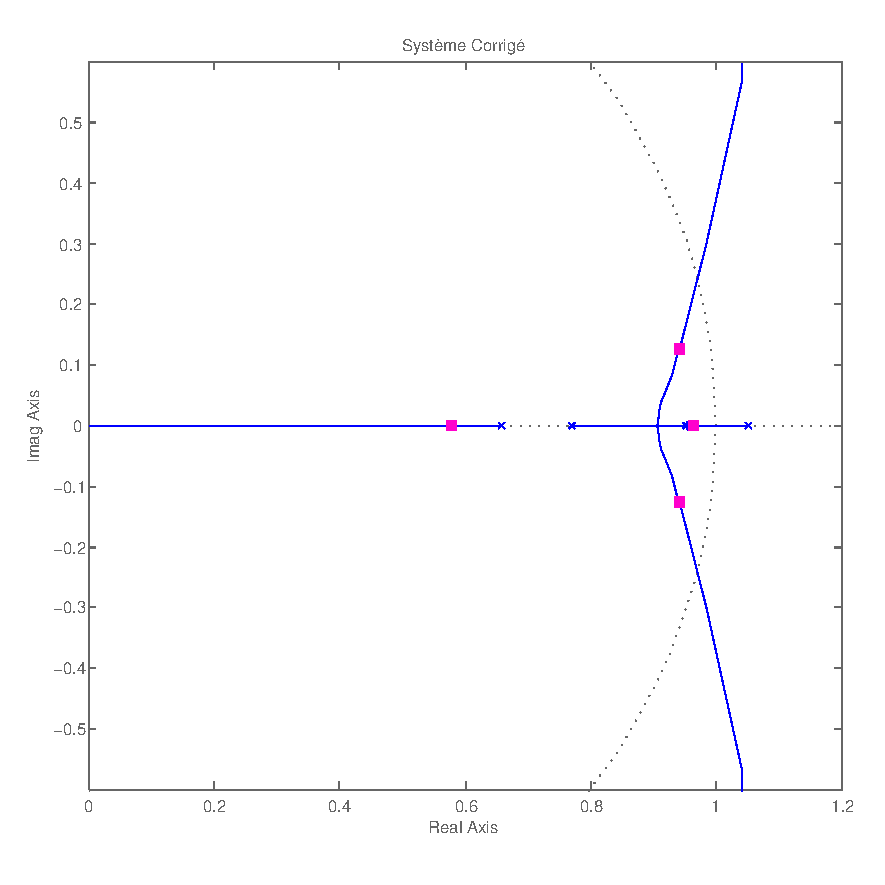
\includegraphics[scale=0.50]{RLN_Sys_AvPh_K5.pdf}

\section{Correcteur numérique}
\section{Conclusion}





\end{document}
